
%(BEGIN_QUESTION)
% Copyright 2010, Tony R. Kuphaldt, released under the Creative Commons Attribution License (v 1.0)
% This means you may do almost anything with this work of mine, so long as you give me proper credit

Suppose a FOUNDATION Fieldbus pressure transmitter will be used to measure vacuum in a process vessel.  The transmitter will be connected to the vessel through an impulse line connected to the ``High'' port.  The operator, in turn, expects to be able to read vacuum as a negative pressure value (i.e. a vacuum of 5 PSI registers as -5 PSI on the operator's display):

$$\includegraphics[width=15.5cm]{i04593x01.eps}$$

The desired measurement range for this transmitter is 0 PSI to -12 PSI.  Complete the configuration table in the above illustration, showing the proper {\tt XD\_Scale}, {\tt OUT\_Scale}, and {\tt L\_Type} parameter values to make the transmitter function as it should in this application.

\vskip 10pt

Also, determine the proper settings (open or shut) for the three hand valves between the process vessel and the transmitter while the system is operating normally.

\vskip 20pt \vbox{\hrule \hbox{\strut \vrule{} {\bf Suggestions for Socratic discussion} \vrule} \hrule}

\begin{itemize}
\item{} Explain why process transmitters with analog (4-20 mA) outputs do not have {\tt XD\_Scale} and {\tt OUT\_Scale} parameters like Fieldbus transmitters.
\end{itemize}

\underbar{file i04593}
%(END_QUESTION)





%(BEGIN_ANSWER)

The {\tt L\_Type} parameter needs to be set to ``Direct''.

%(END_ANSWER)





%(BEGIN_NOTES)

{\tt L\_Type} = Direct

\vskip 10pt

{\tt XD\_Scale} = 0 to -12 PSI

\vskip 10pt

{\tt OUT\_Scale} = 0 to -12 PSI

%INDEX% Fieldbus, instrument ranging: setting XD_Scale and OUT_Scale parameters for an application

%(END_NOTES)

